\chapter{Results}
\label{chap:results}

This chapter answers the questions of the thesis with the results of the simulations. It first checks that
the implementation behaves like the scheme it reproduces (Section~\ref{sec:res-replication}) and explains
how the configuration of the experiments was chosen (Section~\ref{sec:res-diagnosis}). It then evaluates the
two design changes of this thesis, the individual reward (Section~\ref{sec:res-reward}) and gossip
aggregation (Section~\ref{sec:res-gossip}), first one by one and then together
(Section~\ref{sec:res-combined}). The next four sections look behind the final numbers: how the agents learn
(Section~\ref{sec:res-learning}), what behavior they learn (Section~\ref{sec:res-behavior}), how similar
their models end up (Section~\ref{sec:res-consensus}), and how much communication each form of aggregation
costs (Section~\ref{sec:res-communication}). The chapter closes with a fixed rule that beats every learning
method (Section~\ref{sec:res-threshold}), a discussion (Section~\ref{sec:res-discussion}), and the threats to
validity (Section~\ref{sec:res-threats}).

\paragraph{How to read the numbers.} Four conventions hold throughout the chapter
(Chapter~\ref{chap:experimental-setup} gives the details):
\begin{itemize}[nosep]
  \item \emph{One yardstick for all.} The reward reported is always the shared reward of
    \citet{li+22fedmarl} (Section~\ref{sec:sm-shared-reward}), summed over the 200 slots of an episode.
    This holds even when the agents learned from the individual reward, so every method is judged by the
    same measure. Higher is better, and the reward becomes negative when many pairs miss their constraints.
  \item \emph{Final value.} The final value of a run is its mean reward over the last 200 episodes, the
    last 10\% of training. Unless stated otherwise, each number is a final value averaged over the three
    seeds, and $\pm$ gives the standard deviation across seeds.
  \item \emph{Paired comparisons.} Two runs with the same number of pairs $K$ and the same seed see exactly
    the same scenarios: the same positions and the same fading. ``3/3'' means that a method beat another in
    all three seeds, scenario for scenario.
  \item \emph{Sign test.} If two methods were equally good, each paired comparison would be a coin flip.
    The probability $p$ of a result at least as lopsided as the one observed tells how unlikely it is to be
    due to chance. For example, winning 12 of 12 comparisons has $p = 2^{-12} \approx 2 \times 10^{-4}$.
\end{itemize}

\paragraph{The compared methods.} Five methods appear in the tables and figures
(Section~\ref{sec:exp-methods}). Two are fixed rules that do not learn. In \emph{Greedy}, the reference rule of
\citet{li+22fedmarl}, every pair always transmits at maximum power, on the channel with the fewest
neighboring pairs in the previous slot. In the \emph{threshold rule}, pairs choose their channel in the same
way, but only pairs with a strong link transmit at once; pairs with a weak link stay silent until their queue
is almost full. Three methods learn, all with the same \ac{D3QN} agent. In \ac{DTE}, each agent learns alone
and shares nothing. In \ac{FedAvg}, the \ac{BS} averages the networks of all the agents every 50 slots. In
\emph{gossip}, each agent averages its network only with those of its neighbors, the pairs within
\SI{300}{\meter}. Gossip also appears with at most $S = 2$ or $S = 3$ neighbors per round.

\paragraph{Main findings.} In brief:
\begin{enumerate}[nosep]
  \item Learning from an individual reward makes the whole system better, even when it is judged by the
    shared reward. It won 50 of 54 paired comparisons, and its advantage grows with the number of pairs
    (Section~\ref{sec:res-reward}).
  \item With the individual reward, gossip beats \ac{FedAvg} in all 12 comparisons with 10 to 25 pairs,
    without needing the \ac{BS} (Section~\ref{sec:res-gossip}).
  \item Together, the two changes beat the original scheme in all 18 comparisons
    (Section~\ref{sec:res-combined}).
  \item Limited to two neighbors per round, gossip transfers no more models than \ac{FedAvg}, its busiest
    node carries up to ten times less than the \ac{BS}, and it loses no reward
    (Section~\ref{sec:res-communication}).
  \item A simple fixed rule that uses only local information still beats every learning method, so the
    learned policies are still far from what that information allows (Section~\ref{sec:res-threshold}).
\end{enumerate}

%%
\section{Does the implementation reproduce the original scheme?}
% Comparar la tasa media de los CUE con la Fig. 3 de Li et al. para FedAvg y Greedy y comprobar que se mantienen las tendencias.
\label{sec:res-replication}

Before changing a scheme, it is worth checking that the implementation behaves like it.
Table~\ref{tab:res-replication} compares the mean rate of the \acp{CUE} with the values that
\citet{li+22fedmarl} report in their Fig.~3 for \ac{FedAvg} and for Greedy. The values need not match,
because the channel, the geometry, and the traffic are simplified here (Section~\ref{sec:impl-differences}).
What matters is whether the trends hold.

\begin{table}[tbp]
  \centering
  \small
  \caption[Mean CUE rate compared with Li et al. (2022)]{Mean rate of the \acsp{CUE}, in Mbps, compared
    with Fig.~3 of \citet{li+22fedmarl}, whose values are approximate because they were read from the
    figure. ``Shared'' and ``Individual'' name the reward from which the agents of this thesis learn. The
    last row is the relative change from $K = 5$ to $K = 30$.}
  \label{tab:res-replication}
  \begin{tabular}{@{}lccccc@{}}
    \toprule
    & \multicolumn{3}{c}{\acs{FedAvg}} & \multicolumn{2}{c}{Greedy} \\
    \cmidrule(lr){2-4} \cmidrule(l){5-6}
    $K$ & Li et al. & Shared & Individual & Li et al. & This thesis \\
    \midrule
    \tablerows{tables/res_replication_cue.tex}
    \bottomrule
  \end{tabular}
\end{table}

The trends hold. With Greedy, the rate of the \acp{CUE} collapses as $K$ grows: it falls by 65\% from 5 to
30 pairs, against 70\% in the paper. This is what one expects from a rule in which every pair always
transmits at maximum power. With \ac{FedAvg}, the \acp{CUE} are much better protected. With the individual
reward, their rate falls by 35\%, close to the 41\% of the paper, and it stays above that of Greedy for every
$K$, as in the paper. With the shared reward, it falls by only 14\%, but not because the scheme protects the
\acp{CUE} better: its agents learn to stay silent most of the time (Section~\ref{sec:res-reward}).
\citet{li+22fedmarl} also report that their scheme keeps the \ac{V2V} delay below
\SI{100}{\milli\second}; here, the mean delay of every learning method lies between 1 and
\SI{30}{\milli\second} (Section~\ref{sec:res-behavior}).

\begin{keyidea}
  The implementation reproduces the qualitative behavior of the original scheme: learning protects the
  \acsp{CUE} much better than the greedy rule, and the advantage grows with the number of pairs. All the
  comparisons that follow are made within the same simulator, so they do not depend on the absolute values
  matching those of the paper.
\end{keyidea}

%%
\section{Diagnosis: why the original scheme degrades}
% Por qué el esquema original olvida lo aprendido cuando termina la exploración con gamma = 0.99, y cómo el diagnóstico llevó a la configuración de los barridos.
\label{sec:res-diagnosis}

The first runs of the original scheme, with $\gamma = 0.99$, showed a problem that the paper does not report:
the reward rises during the first half of training and then drops when exploration reaches its floor, at
episode 1200. With $K = 10$ and seed 0, \ac{FedAvg} reaches 4526 in its best block of 200 episodes and ends
at 3226, 29\% lower (Figure~\ref{fig:res-diagnosis}, gray line). Greedy, in the same scenarios, obtains
5369: the learning scheme ends far below the simplest rule. A diagnosis looked for the cause with 24
variants, organized in six sets, each one asking a single question (Table~\ref{tab:res-diagnosis}). All of
them use \ac{FedAvg}, $K = 10$, and seed 0.

\begin{figure}[tbp]
  \centering
  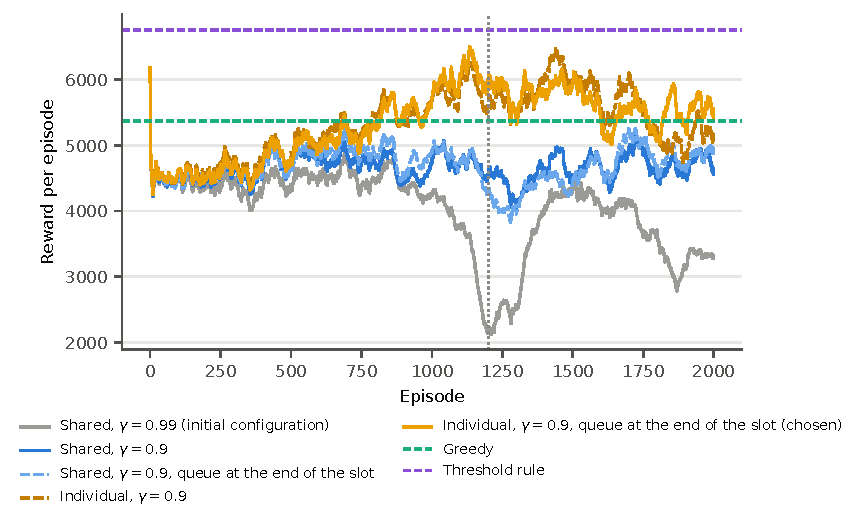
\includegraphics[width=\linewidth]{figures/res_diagnosis.pdf}
  \caption[Diagnosis: learning curves of five variants]{Learning curves of five variants of the diagnosis
    (\acs{FedAvg}, $K = 10$, seed 0), smoothed with a moving average of 50 episodes. The horizontal lines
    are Greedy and the threshold rule in the same scenarios. The dotted vertical line marks episode 1200,
    where exploration reaches its floor.}
  \label{fig:res-diagnosis}
\end{figure}

\begin{table}[tbp]
  \centering
  \small
  \caption[Results of the diagnosis]{Diagnosis of training (\acs{FedAvg}, $K = 10$, seed 0). ``Peak'' is
    the best mean over a block of 200 episodes, ``Final'' the mean over the last 200, and ``Change'' the
    relative difference between them. The groups are, in order, the sets on the drop, learning, $\gamma$,
    the queue, the reward, and stability. In bold, the chosen configuration. With the same seed, Greedy
    obtains 5369 and the threshold rule 6754.}
  \label{tab:res-diagnosis}
  \begin{tabularx}{\textwidth}{@{}llXrrr@{}}
    \toprule
    Reward & $\gamma$ & Other changes & Peak & Final & Change \\
    \midrule
    \tablerows{tables/res_diagnosis.tex}
    \bottomrule
  \end{tabularx}
\end{table}

\paragraph{Drop: too little memory or too large a scale?} Two common stabilizers soften the drop without
solving the problem. A replay buffer ten times larger, which holds 500 episodes instead of 50, reduces it to
6\%, and multiplying the reward by 0.01, so that the Q values are smaller, reduces it to 20\%. With both
changes at once, the variant ends at 4411, still far below Greedy.

\paragraph{Learning: is it the differences from the paper?} The network of \citet{li+22fedmarl}, with layers
of 500, 250, and 120 neurons, ends at 3788, and their exploration floor of 0.1 ends at 3739. Both end
somewhat better than the initial configuration, but neither avoids the drop (17\% and 19\% below their
peaks). The differences in configuration from the paper do not explain the problem.

\paragraph{The discount factor.} The change that almost removes the drop is lowering $\gamma$ from 0.99 to
0.9: the variant ends at 4703, only 3\% below its peak. Nearby values confirm it: 0.85 ends at 4653, 0.8 and
0.7 end lower (4320 and 4263), and 0.95 drops again (3329). A possible explanation lies in the scale of the
Q values. With $\gamma = 0.99$, the return weighs about 100 future slots, the horizon $1/(1-\gamma)$ of
Section~\ref{sec:bg-rl}, so the Q values are about a hundred times the reward of one slot. The difference
between staying silent and transmitting in one slot is a tiny fraction of them, and it gets lost in the
estimation error. With $\gamma = 0.9$, the horizon is about 10 slots, and that difference weighs ten times
more. Since \citet{li+22fedmarl} do not give the value of $\gamma$, choosing 0.9 does not depart from the
paper.

\paragraph{Queue: does it matter when the cost is charged?} With the shared reward, measuring the queue at
the end of the slot instead of at its start does not change the result. With $\gamma = 0.99$, the variant
drops just the same (3343), and with $\gamma = 0.9$ it ends at 4852, practically the same as without the
change. Adding to the observation the channel that the pair used in the previous slot does not help
consistently either.

\paragraph{Reward: the largest change.} The four variants with the individual reward end above all the
variants with the shared reward, and three of them exceed Greedy in their best stretch (peaks of 5788 to
6051). The best one combines the individual reward, $\gamma = 0.9$, and the queue measured at the end of the
slot. It reaches 6051 and ends at 5586, the first configuration that ends above Greedy. With the individual
reward, measuring the queue at the end of the slot does matter (5586 against 5083). This agrees with the
argument of Section~\ref{sec:pa-individual-reward}: when an agent is judged by its own queue, charging the
cost in the same slot as the action that caused it makes the link between the two clearer.

\paragraph{Stability: can forgetting be avoided?} The best variant still loses 8\% after its peak. On top of
it, a lower learning rate ($3 \times 10^{-4}$ or $10^{-4}$), an exploration floor of 0.1, and a buffer of
100,000 transitions do not improve the final value: the four end between 5126 and 5391. The learning rate of
$3 \times 10^{-4}$ reaches the highest peak, 6234, but forgets just the same.

\paragraph{The chosen configuration.} The sweeps use $\gamma = 0.9$ with both rewards. With the individual
reward, the queue is measured at the end of the slot. With the shared reward, it is measured at the start,
as in \citet{li+22fedmarl}, because measuring it at the end did not change its result. Everything else stays
as in Section~\ref{sec:exp-parameters}.

\paragraph{Two caveats.} First, the diagnosis uses a single seed, and the variability between runs is large.
The chosen configuration, run again with the same seed in the sweep, ended at 4631 instead of 5586. The
diagnosis ran on a graphics card and the sweep on processors; floating-point computations differ slightly
between the two, and these differences are enough for two trainings to take different paths. For this
reason, the diagnosis only served to choose the configuration, and the conclusions of the following sections
rest on the sweeps, with three seeds. Second, in the variants that measure the queue at the end of the slot,
the reward was logged with that same change. The difference is small: the logged reward contains the same
queue terms, shifted by one slot, and it differs from the shared reward as defined by at most 55 per episode
with $K = 10$, about 1\% of the values in the table.

\begin{keyidea}
  The original scheme forgot what it had learned when exploration ended and finished below Greedy. Lowering
  the discount factor to 0.9 almost removed the drop, but only the individual reward took the agents above
  Greedy.
\end{keyidea}

%%
\section{Individual reward versus shared reward}
% Comparar los barridos con recompensa individual y compartida, método por método y semilla por semilla.
\label{sec:res-reward}

The first design question is whether the system works better when each agent learns from its own reward
(Section~\ref{sec:pa-individual-reward}) than when all of them learn from the shared reward
(Section~\ref{sec:sm-shared-reward}). The short answer is yes. Table~\ref{tab:res-shared-individual} and
Figure~\ref{fig:res-individual-shared} compare the two sweeps, which differ only in that respect.

\begin{table}[tbp]
  \centering
  \footnotesize
  \setlength{\tabcolsep}{2.6pt}
  \caption[Shared reward versus individual reward]{Final reward according to the reward from which the
    agents learn. ``Sh.'' and ``Ind.'': learning from the shared and from the individual reward. ``Diff.'':
    individual minus shared. ``Seeds'': seeds in which the individual reward beats the shared one, in the
    same scenarios. Greedy does not learn and is shown as a reference.}
  \label{tab:res-shared-individual}
  \begin{tabular}{@{}r rrrr rrrr rrrr r@{}}
    \toprule
    & \multicolumn{4}{c}{\acs{DTE}} & \multicolumn{4}{c}{\acs{FedAvg}} & \multicolumn{4}{c}{Gossip} & \\
    \cmidrule(lr){2-5} \cmidrule(lr){6-9} \cmidrule(lr){10-13}
    $K$ & Sh. & Ind. & Diff. & Seeds & Sh. & Ind. & Diff. & Seeds & Sh. & Ind. & Diff. & Seeds & Greedy \\
    \midrule
    \tablerows{tables/res_shared_vs_individual.tex}
    \bottomrule
  \end{tabular}
\end{table}

\begin{figure}[tbp]
  \centering
  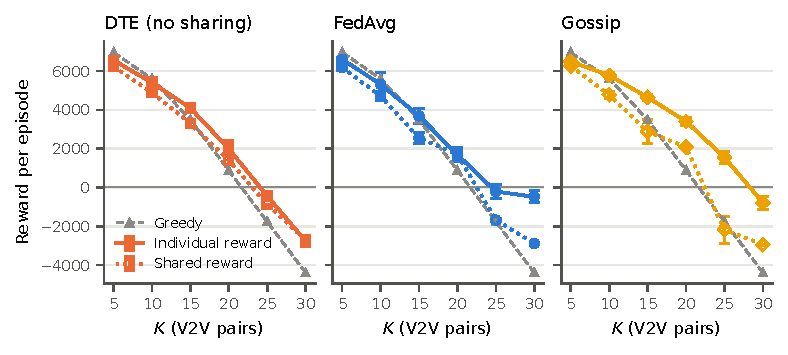
\includegraphics[width=\linewidth]{figures/res_individual_vs_shared.pdf}
  \caption[Individual versus shared reward, per method]{Final reward of each learning method when it
    learns from the individual reward (solid line) or from the shared reward (dotted line), with Greedy as a
    reference. The error bars are the standard deviation across seeds.}
  \label{fig:res-individual-shared}
\end{figure}

\paragraph{The individual reward wins almost always.} In 50 of the 54 paired comparisons (three methods, six
values of $K$, and three seeds), the agents that learn from the individual reward achieve a higher shared
reward than the agents that learn from the shared reward itself ($p \approx 2 \times 10^{-11}$). The four
exceptions are in two cells, \ac{DTE} with $K = 30$ and \ac{FedAvg} with $K = 20$, where the differences
between the means ($-61$ and $-17$) are much smaller than the variability across seeds. With gossip, the
individual reward wins all 18 comparisons.

This result was not obvious in advance. The agents that learn from the shared reward optimize exactly the
measure by which they are judged, and yet they score lower on it than agents that optimize something else.

\paragraph{The gain grows with the number of pairs.} With gossip, the gain goes from 244 with $K = 5$ to
1766 with $K = 15$ and 3726 with $K = 25$; with \ac{FedAvg}, it goes from 421 to 2403 with $K = 30$. This is
what the learnability argument of Section~\ref{sec:bg-marl} predicts. The shared reward adds up $M + 2K$
terms, one for each of the $M = 15$ \acp{CUE} and two for each pair, and the action of one agent directly
affects only a few of them. With more pairs, the signal of each agent is buried deeper in what the others do.

\paragraph{With the shared reward, learning barely beats Greedy.} With $K$ from 5 to 15, the three methods
that learn from the shared reward end below Greedy. They generally beat it only from 20 pairs on, when Greedy
collapses. With the individual reward, by contrast, gossip beats Greedy from $K = 10$ on
(Section~\ref{sec:res-gossip}).

\paragraph{Silence as a strategy.} The behavior of the agents explains much of the difference. With the
shared reward and many pairs, \ac{FedAvg} and gossip learn to stay silent almost always. With $K = 25$, their
pairs miss the reliability condition in 92\% to 93\% of the slots and transmit, on average, at a fifth of the
maximum power, while the \acp{CUE} keep 7.2 to \SI{7.4}{Mbps}, almost as much as with $K = 5$. These are the
lazy agents of \citet{sunehag+18vdn}. Silence protects the \acp{CUE}, which weigh in everyone's reward, while
its cost, the reliability of the pair itself, is only one of the 65 terms of the reward. In the individual
reward, that cost is one of only three terms, and the pairs transmit more: with $K = 25$, their outage falls
to 71\%--77\%.

\paragraph{More stable curves.} The learning curves with the shared reward
(Figure~\ref{fig:res-curves-shared}) are irregular and often drop when exploration ends. \ac{FedAvg} with
$K = 15$ goes from about 3300 to about 2300 around episode 1200, and gossip with $K = 25$ drops near the end
from about 0 to about $-3000$. With the individual reward (Figure~\ref{fig:res-curves-individual}, in the
next section), the curves of gossip rise more steadily and keep what they gain
(Section~\ref{sec:res-learning}).

\begin{figure}[tbp]
  \centering
  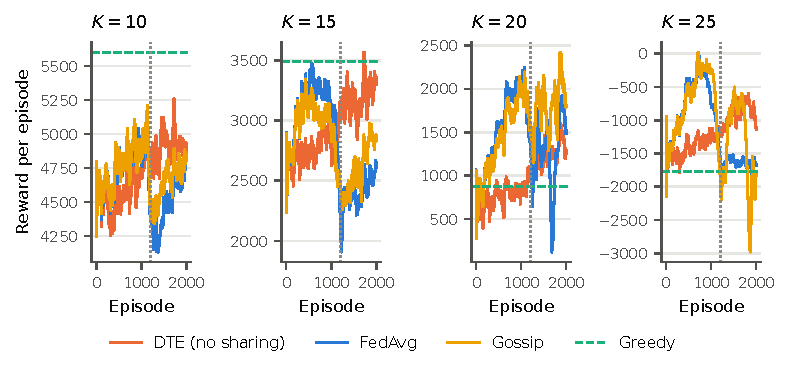
\includegraphics[width=\linewidth]{figures/res_curves_shared.pdf}
  \caption[Learning curves with the shared reward]{Learning curves with the shared reward: mean of the three
    seeds, smoothed with a moving average of 50 episodes. The horizontal line is Greedy, and the dotted
    vertical line marks episode 1200, where exploration ends. The vertical scales differ between panels.}
  \label{fig:res-curves-shared}
\end{figure}

\begin{keyidea}
  When each agent learns from its own reward, the system works better, even when it is judged by everyone's
  reward. The individual reward won 50 of 54 comparisons, including all those of gossip, and its advantage
  grows with the number of pairs. With the shared reward, the agents tend to stay silent.
\end{keyidea}

%%
\section{Gossip aggregation versus FedAvg}
% Recompensa final de todos los métodos con la recompensa individual y comparación de gossip con cada uno, semilla por semilla.
\label{sec:res-gossip}

The second design question is whether the agents learn better by averaging their models with those of their
neighbors than with those of all the agents through the \ac{BS}. With the individual reward, the answer is
yes for 10 to 25 pairs. Table~\ref{tab:res-reward} and Figure~\ref{fig:res-reward-k} show the final reward
of every method with the individual reward, and Table~\ref{tab:res-wins} compares gossip with each of the
others, seed by seed.

\begin{table}[tbp]
  \centering
  \small
  \caption[Final reward with the individual reward]{Final reward of each method (mean $\pm$ standard
    deviation across seeds), with the agents learning from the individual reward. In bold, the best of the
    learning methods.}
  \label{tab:res-reward}
  \begin{tabular}{@{}rrrrrr@{}}
    \toprule
    $K$ & Threshold rule & Greedy & \acs{DTE} & \acs{FedAvg} & Gossip \\
    \midrule
    \tablerows{tables/res_reward_individual.tex}
    \bottomrule
  \end{tabular}
\end{table}

\begin{figure}[tbp]
  \centering
  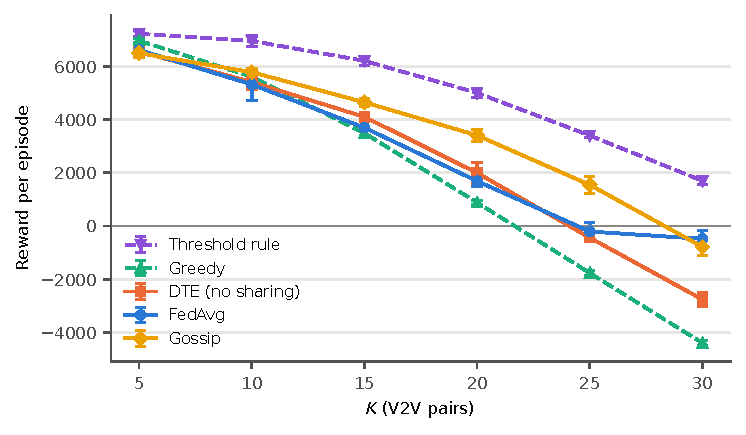
\includegraphics{figures/res_reward_vs_k.pdf}
  \caption[Final reward against the number of pairs]{Final reward against the number of pairs, with the
    agents learning from the individual reward. The dashed lines are the rules that do not learn, and the
    error bars are the standard deviation across seeds.}
  \label{fig:res-reward-k}
\end{figure}

\begin{table}[tbp]
  \centering
  \small
  \caption[Gossip against the other methods]{Gossip against the other methods. ``Diff.'': difference
    between the mean final rewards (gossip minus the other method). ``Seeds'': seeds in which gossip beats
    the other method in the same scenarios.}
  \label{tab:res-wins}
  \begin{tabular}{@{}r rr rr rr rr@{}}
    \toprule
    & \multicolumn{6}{c}{Individual reward} & \multicolumn{2}{c}{Shared reward} \\
    \cmidrule(lr){2-7} \cmidrule(l){8-9}
    & \multicolumn{2}{c}{against \acs{FedAvg}} & \multicolumn{2}{c}{against \acs{DTE}}
      & \multicolumn{2}{c}{against Greedy} & \multicolumn{2}{c}{against \acs{FedAvg}} \\
    \cmidrule(lr){2-3} \cmidrule(lr){4-5} \cmidrule(lr){6-7} \cmidrule(l){8-9}
    $K$ & Diff. & Seeds & Diff. & Seeds & Diff. & Seeds & Diff. & Seeds \\
    \midrule
    \tablerows{tables/res_gossip_wins.tex}
    \bottomrule
  \end{tabular}
\end{table}

\paragraph{Gossip beats FedAvg in the middle range.} With $K$ between 10 and 25, gossip achieves the highest
reward of the learning methods and beats \ac{FedAvg} in all 12 paired comparisons
($p \approx 2 \times 10^{-4}$). Its advantage grows with the number of pairs: 459 with $K = 10$, 956 with
$K = 15$, 1717 with $K = 20$, and 1754 with $K = 25$. Counting all six values of $K$, gossip wins 14 of 18
comparisons ($p \approx 0.015$).

\paragraph{At the extremes, the advantage disappears.} With $K = 5$, the three learning methods end within
120 of each other, inside the variability across seeds. With so few pairs, 31\% of them have no neighbor at
all in a given episode (Section~\ref{sec:res-consensus}), so gossip shares little. With $K = 30$, \ac{FedAvg}
beats gossip by 304 and wins in two of the three seeds. The gossip variant with $S = 2$, however, beats
\ac{FedAvg} in all three (Section~\ref{sec:res-communication}).

\paragraph{Sharing with neighbors helps; sharing with everyone does not always.} Against \ac{DTE}, which
shares nothing, gossip wins 16 of the 18 comparisons, including all 15 from $K = 10$ on, with advantages from
372 to 1986. \ac{FedAvg}, by contrast, beats \ac{DTE} in only 9 of 18. With $K$ from 10 to 20, averaging with
all the agents of the cell gives the same result as not sharing, or a worse one (differences of $-88$,
$-406$, and $-308$); it helps only with 25 and 30 pairs. Sharing by itself is not enough: whom an agent shares
with matters.

\paragraph{Gossip beats the rule of the paper.} Against Greedy, gossip loses with $K = 5$. With so few pairs
there is little interference, and always transmitting at maximum power is nearly the best one can do. From
$K = 10$ on, gossip wins all 15 comparisons, with advantages that grow from 172 to 3608.

\paragraph{With the shared reward, the aggregation makes no difference.} If the agents learn from the shared
reward, gossip and \ac{FedAvg} tie. Gossip wins 10 of 18 comparisons ($p \approx 0.41$), with differences
between $-499$ and $+380$ (last columns of Table~\ref{tab:res-wins}). The advantage of gossip appears only
when each agent learns from its own reward. Section~\ref{sec:res-discussion} proposes an explanation.

\paragraph{The learning curves.} Figure~\ref{fig:res-curves-individual} shows how the rewards evolve with the
individual reward. \ac{FedAvg} rises quickly at first, but with $K = 20$ and $K = 25$ it drops when
exploration ends. Gossip rises more slowly, keeps what it gains, and from $K = 15$ on ends clearly above the
others.

\begin{figure}[tbp]
  \centering
  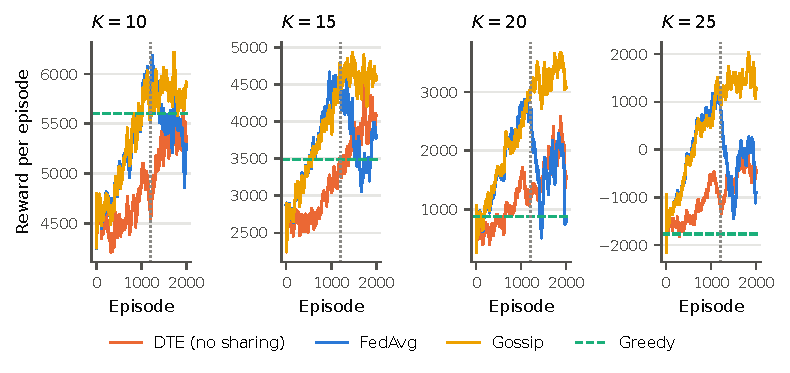
\includegraphics[width=\linewidth]{figures/res_curves_individual.pdf}
  \caption[Learning curves with the individual reward]{Learning curves with the individual reward: mean of
    the three seeds, smoothed with a moving average of 50 episodes. The horizontal line is Greedy, and the
    dotted vertical line marks episode 1200, where exploration ends.}
  \label{fig:res-curves-individual}
\end{figure}

\begin{keyidea}
  With the individual reward, averaging with neighbors works better than averaging with everyone through
  the \acs{BS}. Gossip beat \acs{FedAvg} in all 12 comparisons with 10 to 25 pairs, and beat not sharing in
  16 of 18, without needing the \acs{BS}.
\end{keyidea}

%%
\section{The complete proposal versus the original scheme}
% La propuesta (gossip con recompensa individual) y su variante con S = 2 frente al esquema original (FedAvg con recompensa compartida).
\label{sec:res-combined}

The two previous sections evaluate each change on its own. Table~\ref{tab:res-combined} evaluates them
together: it compares the original scheme of \citet{li+22fedmarl}, \ac{FedAvg} with the shared reward, with
the proposal of this thesis, gossip with the individual reward, and with its variant of bounded cost,
$S = 2$.

\begin{table}[tbp]
  \centering
  \small
  \caption[The proposal versus the original scheme]{The proposal against the original scheme. ``Diff.'':
    difference between the mean final rewards, relative to the original scheme. ``Seeds'': seeds in which
    the proposal beats the original scheme in the same scenarios.}
  \label{tab:res-combined}
  \begin{tabular}{@{}r r rrr rrr@{}}
    \toprule
    & Original scheme & \multicolumn{3}{c}{Gossip, individual reward}
      & \multicolumn{3}{c}{Gossip with $S = 2$, individual} \\
    \cmidrule(lr){3-5} \cmidrule(l){6-8}
    $K$ & \acs{FedAvg}, shared & Reward & Diff. & Seeds & Reward & Diff. & Seeds \\
    \midrule
    \tablerows{tables/res_combined.tex}
    \bottomrule
  \end{tabular}
\end{table}

The proposal beats the original scheme in all 18 paired comparisons, for every $K$ and every seed
($p = 2^{-18} \approx 4 \times 10^{-6}$), with advantages from 306 with $K = 5$ to 3227 with $K = 25$. The
variant with $S = 2$ also wins all 18, with advantages from 341 to 3485, while transferring at most as many
models as \ac{FedAvg} (Section~\ref{sec:res-communication}). In relative terms, with $K = 15$ the proposal
achieves 1.8 times the reward of the original scheme, and with $K = 25$ it goes from a negative reward,
$-1682$, to a positive one, 1545.

\begin{keyidea}
  Gossip with the individual reward beat the original scheme in every scenario, and its advantage grows with
  the number of pairs.
\end{keyidea}

%%
\section{Learning speed and stability}
% Cuánto mejora cada método, en qué episodio alcanza el 90 % de esa mejora y cuánto pierde al final del entrenamiento.
\label{sec:res-learning}

Besides where each method ends, it matters how it gets there. Table~\ref{tab:res-convergence} shows, with the
individual reward, how much each method improves during training and at which episode it reaches 90\% of
that improvement. Table~\ref{tab:res-forgetting} shows how much each method loses after its best stretch.

\begin{table}[tbp]
  \centering
  \small
  \caption[Speed and size of learning]{Speed and size of learning with the individual reward. The
    improvement is the final value minus the mean of the first 50 episodes. The episode is the first one at
    which the moving average over 50 episodes covers 90\% of that improvement (mean of the three seeds).}
  \label{tab:res-convergence}
  \begin{tabular}{@{}r rrr rrr@{}}
    \toprule
    & \multicolumn{3}{c}{Episode at 90\% of the improvement} & \multicolumn{3}{c}{Improvement} \\
    \cmidrule(lr){2-4} \cmidrule(l){5-7}
    $K$ & \acs{DTE} & \acs{FedAvg} & Gossip & \acs{DTE} & \acs{FedAvg} & Gossip \\
    \midrule
    \tablerows{tables/res_convergence.tex}
    \bottomrule
  \end{tabular}
\end{table}

\paragraph{FedAvg is the fastest; gossip goes further.} \ac{FedAvg} reaches 90\% of its improvement before
the others: between episodes 411 and 562 for $K$ from 5 to 25. Gossip takes longer, between 765 and 1170
episodes for $K$ from 10 to 25, and \ac{DTE} is usually the slowest. But gossip improves much more: for $K$
from 10 to 25, its improvement is 1.6 to 2.6 times that of \ac{FedAvg}. The speed of \ac{FedAvg} has a direct
explanation. After each round, all the agents have the same model, so what one agent learns reaches all the
others at once. In gossip, knowledge advances one neighbor per round and takes time to cross the cell, as
Section~\ref{sec:bg-dfl} anticipates.

\paragraph{FedAvg forgets; gossip keeps.} With the individual reward and $K$ from 10 to 25, \ac{FedAvg} loses
between 551 and 1270 after its best stretch, while gossip loses at most 154 (Table~\ref{tab:res-forgetting}).
With the shared reward, \ac{FedAvg} forgets similar amounts, and gossip forgets considerably more: up to 2318
with $K = 25$. \ac{DTE} forgets little, but only because it improves so slowly that its best episodes are
usually the last ones.

\begin{table}[tbp]
  \centering
  \small
  \caption[Forgetting at the end of training]{Forgetting: the best mean over a block of 200 episodes minus the
    mean over the last 200 (mean of the three seeds). A zero means that the last block was the best one.}
  \label{tab:res-forgetting}
  \begin{tabular}{@{}r rrr rrr@{}}
    \toprule
    & \multicolumn{3}{c}{Shared reward} & \multicolumn{3}{c}{Individual reward} \\
    \cmidrule(lr){2-4} \cmidrule(l){5-7}
    $K$ & \acs{DTE} & \acs{FedAvg} & Gossip & \acs{DTE} & \acs{FedAvg} & Gossip \\
    \midrule
    \tablerows{tables/res_forgetting.tex}
    \bottomrule
  \end{tabular}
\end{table}

\paragraph{No curve fully settles.} Only 19 of the 54 runs of the learning methods with the individual reward
end within a band of $\pm 5\%$ around their final value, and none before episode 1789. The curves keep moving
until the end: exploration never stops completely ($\varepsilon = 0.05$), and each agent keeps adapting to
the others, which also keep changing. For this reason, this thesis compares final values rather than
``episodes to convergence''.

\begin{keyidea}
  \acs{FedAvg} learns fastest, because every round gives all the agents the same model, but it loses part of
  what it learned when exploration ends. Gossip learns more slowly, improves much more, and keeps what it
  learns.
\end{keyidea}

%%
\section{What the agents learn}
% Medidas de calidad de servicio y de comportamiento (qué canales y potencias eligen) que explican las diferencias en la recompensa.
\label{sec:res-behavior}

The reward sums up performance in a single number. The measures of quality of service
(Figure~\ref{fig:res-qos}) and of behavior (Figure~\ref{fig:res-behavior}) show what lies behind it.
Appendix~\ref{apx:detailed-results} gives the complete tables, for both rewards.

\begin{figure}[tbp]
  \centering
  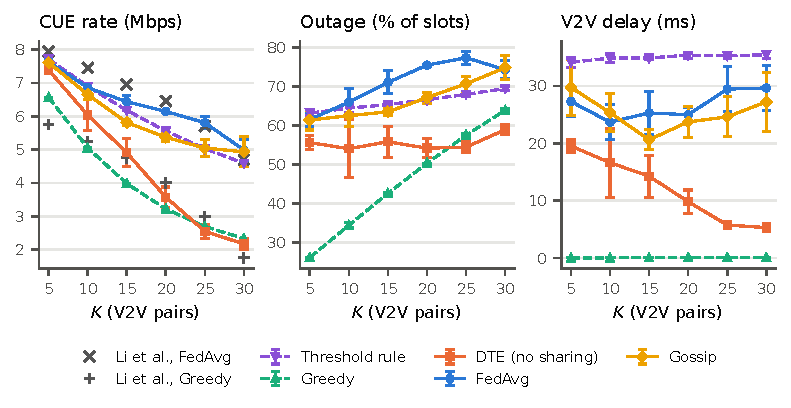
\includegraphics[width=\linewidth]{figures/res_qos.pdf}
  \caption[Quality of service with the individual reward]{Quality of service with the individual reward:
    mean rate of the \acsp{CUE} (with the values of Fig.~3 of \citet{li+22fedmarl}), percentage of slots
    in outage, and mean delay of the pairs. A slot in which the pair stays silent counts as an outage.}
  \label{fig:res-qos}
\end{figure}

\begin{figure}[tbp]
  \centering
  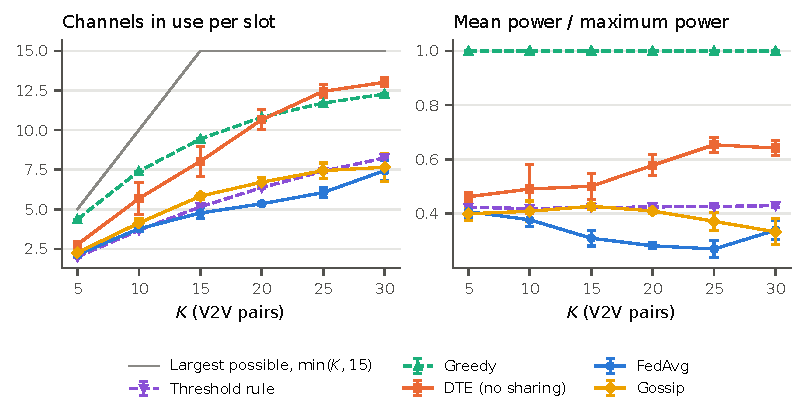
\includegraphics[width=\linewidth]{figures/res_behavior.pdf}
  \caption[Use of the spectrum with the individual reward]{Use of the spectrum with the individual reward:
    number of different channels used by the pairs that transmit, and mean transmit power as a fraction of
    the maximum.}
  \label{fig:res-behavior}
\end{figure}

\paragraph{Greedy saturates the spectrum.} Greedy always transmits at maximum power and occupies many
channels, from 4.4 with $K = 5$ to 12.3 with $K = 30$. With 30 pairs, 87\% of the time it shares its channel
with another pair that transmits. Its delay is zero, because it is never silent, but the interference brings
down the rate of the \acp{CUE}, from 6.6 to \SI{2.3}{Mbps}, and the reliability of its own links: its outage
rises from 26\% to 64\%.

\paragraph{The methods that share learn to be cautious.} With \ac{FedAvg} and gossip, the pairs transmit, on
average, at 27\% to 43\% of the maximum power and occupy few channels, at most 7.7 of the 15. This protects
the \acp{CUE}: with 30 pairs, their rate is about \SI{5}{Mbps}, more than twice that with Greedy. The price
is a delay of 20 to \SI{30}{\milli\second} and an outage of 61\% to 77\%, much of which corresponds to
silent slots. In all cases, the delay stays far below the maximum of \SI{100}{\milli\second}. Why the agents
concentrate their transmissions on a few channels was not studied in this thesis. One possibility is that
they choose the channels whose \acp{CUE} have a better link to the \ac{BS}, which the observation includes,
because those \acp{CUE} tolerate more interference.

\paragraph{DTE becomes aggressive.} Without sharing, the agents end up behaving much like Greedy when there
are many pairs. With $K = 30$, they transmit at 64\% of the maximum power, occupy 13 channels, share a channel
62\% of the time, and leave the \acp{CUE} with \SI{2.2}{Mbps}, less than Greedy. Their delay is low
(\SI{5}{\milli\second}), but the interference they cause weighs more in the reward.

\paragraph{Outage is misleading.} The method with the lowest outage is Greedy, which is the worst for the
\acp{CUE}. Because silence counts as outage, this measure punishes caution, and it cannot rank the methods
on its own. The reward, which weighs the three objectives, can.

\begin{keyidea}
  Greedy and \acs{DTE} transmit aggressively and drown the \acsp{CUE} in interference. The agents of
  \acs{FedAvg} and gossip learn to transmit at moderate power on a few channels, which protects the
  \acsp{CUE} at the price of a delay that stays well within its limit.
\end{keyidea}

%%
\section{Neighborhoods and consensus}
% Número de vecinos según K, pares aislados y qué tan parecidos terminan los modelos de los agentes con gossip.
\label{sec:res-consensus}

How well gossip works depends on how many neighbors each vehicle has. Figure~\ref{fig:res-topology} shows
that the mean number of neighbors grows linearly with $K$, from 1.07 with $K = 5$ to 7.80 with $K = 30$. Each
pair has, on average, $0.27\,(K - 1)$ neighbors. A pair far from the edge of the cell would have $0.36\,(K - 1)$,
since a circle of \SI{300}{\meter} covers $(300/500)^2 = 0.36$ of the cell; pairs near the edge have fewer.
With few pairs, many are isolated: 31\% with $K = 5$, 8\% with $K = 10$, and less than 1\% from $K = 20$ on.

\begin{figure}[tbp]
  \centering
  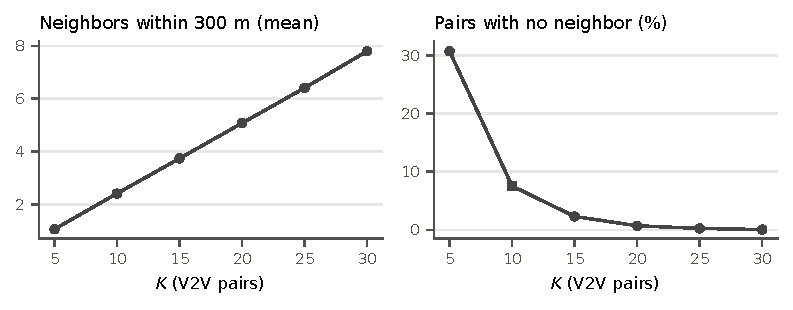
\includegraphics[width=\linewidth]{figures/res_topology.pdf}
  \caption[Neighborhoods against the number of pairs]{Mean number of neighbors of a pair (transmitters at
    most \SI{300}{\meter} apart) and percentage of pairs with no neighbor, against the number of pairs.}
  \label{fig:res-topology}
\end{figure}

How similar do the models of the agents end up? Figure~\ref{fig:res-dispersion} shows the \termdef{weight
dispersion}: the mean distance between the weights of each agent and the average of the weights of all the
agents, measured right before each round. Without sharing (\ac{DTE}), the dispersion is 170 to 240: the agents
start from different random weights and never come closer. With \ac{FedAvg}, it is 0.7 to 0.9, the distance
the agents drift apart in the 50 slots that follow each round. With gossip, it is 0.95 to 1.65, two orders of
magnitude smaller than without sharing and of the same order as with \ac{FedAvg}, even though each agent only
averages with its neighbors. This is the consensus of Section~\ref{sec:bg-dfl} at work: since the
neighborhoods change in every episode, what each agent knows ends up reaching all the others. The
dispersion of gossip is larger with few pairs, when more of them are isolated, and it falls as the graph
becomes denser.

\begin{figure}[tbp]
  \centering
  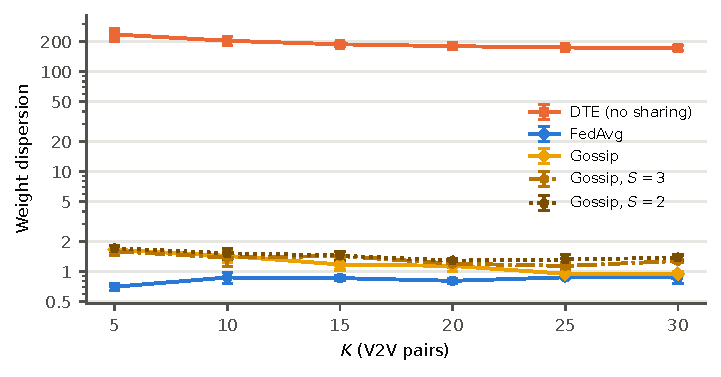
\includegraphics{figures/res_dispersion.pdf}
  \caption[Weight dispersion]{Dispersion of the weights of the agents, measured before each round
    (logarithmic scale). Zero would mean that all the agents have exactly the same model.}
  \label{fig:res-dispersion}
\end{figure}

\begin{keyidea}
  Even though each agent only averages with its neighbors, the models of gossip end up almost as close to
  each other as those of \acs{FedAvg}, and a hundred times closer than without sharing.
\end{keyidea}

%%
\section{Communication cost}
% Modelos transferidos y carga del nodo más cargado por episodio con cada forma de agregación, comparados con FedAvg.
\label{sec:res-communication}

Table~\ref{tab:res-communication} and Figure~\ref{fig:res-communication} measure the cost of each form of
aggregation with two numbers (Section~\ref{sec:pa-comm-cost}): the models transferred in an episode, and the
transfers in which the busiest node takes part.

\begin{table}[tbp]
  \centering
  \footnotesize
  \setlength{\tabcolsep}{3pt}
  \caption[Communication cost per episode]{Communication cost per episode (four rounds): models transferred
    and load of the busiest node, which in \acs{FedAvg} is always the \acs{BS}. The ratio columns divide by
    the value of \acs{FedAvg}.}
  \label{tab:res-communication}
  \begin{tabular}{@{}r rrrr rr rrr rr@{}}
    \toprule
    & \multicolumn{6}{c}{Models transferred} & \multicolumn{5}{c}{Load of the busiest node} \\
    \cmidrule(lr){2-7} \cmidrule(l){8-12}
    $K$ & \acs{FedAvg} & Gossip & $S{=}3$ & $S{=}2$ & \makecell{Gossip/\\\acs{FedAvg}}
      & \makecell{$S{=}2$/\\\acs{FedAvg}} & \acs{FedAvg} & Gossip & $S{=}2$
      & \makecell{Gossip/\\\acs{FedAvg}} & \makecell{$S{=}2$/\\\acs{FedAvg}} \\
    \midrule
    \tablerows{tables/res_communication.tex}
    \bottomrule
  \end{tabular}
\end{table}

\begin{figure}[tbp]
  \centering
  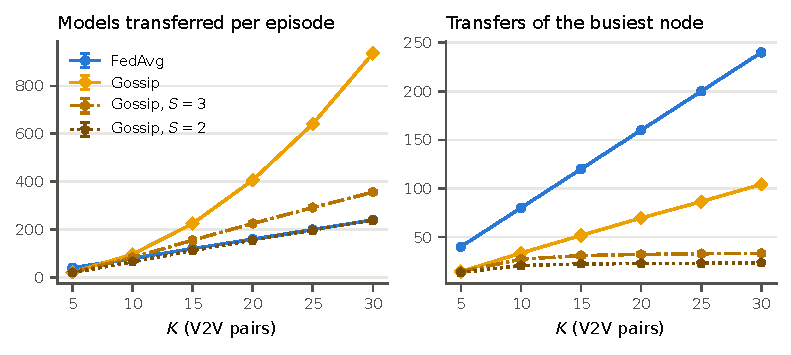
\includegraphics[width=\linewidth]{figures/res_communication.pdf}
  \caption[Communication cost against the number of pairs]{Models transferred per episode (left) and
    transfers of the busiest node (right). In \acs{FedAvg}, the busiest node is the \acs{BS}.}
  \label{fig:res-communication}
\end{figure}

\paragraph{With all neighbors, the total grows with the square of $K$.} \ac{FedAvg} transfers $8K$ models per
episode, from 40 to 240: in each of the four rounds, every pair sends its model to the \ac{BS} and receives
the average. Gossip with all its neighbors transfers 21 with $K = 5$, half as many as \ac{FedAvg}, but from
$K = 10$ on it transfers more, and with $K = 30$ it transfers 936, 3.9 times more. The reason is that each of
the $K$ pairs receives a model from each of its $0.27\,(K-1)$ neighbors in every round, which gives
$4 \times 0.27 \times 30 \times 29 \approx 940$ per episode with $K = 30$. In megabytes, \ac{FedAvg} moves
4.9 to \SI{29.2}{\mega\byte} per episode, and gossip 2.6 to \SI{113.8}{\mega\byte}.

\paragraph{No node carries everything.} Although the total is larger, gossip spreads the load. Its busiest
node takes part in 14 to 104 transfers per episode, 36\% to 43\% of what the \ac{BS} handles in \ac{FedAvg}.
And the transfers of gossip travel over the direct link between vehicles, without going through the cellular
network.

\paragraph{Limiting the neighbors bounds the cost without losing reward.} With at most $S = 2$ neighbors per
round, the total never exceeds that of \ac{FedAvg} (between 50\% and 100\% of it), and the load of the
busiest node stops growing. It stays at about 23 transfers per episode from $K = 15$ on, a tenth of the load
of the \ac{BS} with $K = 30$. The reward does not suffer (Table~\ref{tab:res-neighbors}). With $K$ from 10 to
25, the variants with $S = 2$ and $S = 3$ end within about 300 of gossip with all its neighbors, above or
below it, and with $K = 30$ the variant with $S = 2$ is the best of the learning methods (397, against $-484$
for \ac{FedAvg}). Overall, $S = 2$ beats \ac{FedAvg} in 16 of the 18 comparisons
($p \approx 7 \times 10^{-4}$). That averaging with fewer neighbors does not hurt suggests that what matters
is not how many models an agent receives, but that they come from the area where the agent operates.

\begin{table}[tbp]
  \centering
  \small
  \caption[Gossip with at most S neighbors]{Gossip with all its neighbors and with at most $S$ neighbors per
    round, against \acs{FedAvg}, with the individual reward: final reward (mean $\pm$ standard deviation) and
    seeds in which each variant beats \acs{FedAvg} in the same scenarios.}
  \label{tab:res-neighbors}
  \begin{tabular}{@{}r rrrr rrr@{}}
    \toprule
    & \multicolumn{4}{c}{Final reward} & \multicolumn{3}{c}{Seeds above \acs{FedAvg}} \\
    \cmidrule(lr){2-5} \cmidrule(l){6-8}
    $K$ & \acs{FedAvg} & Gossip & $S = 3$ & $S = 2$ & Gossip & $S = 3$ & $S = 2$ \\
    \midrule
    \tablerows{tables/res_gossip_neighbors.tex}
    \bottomrule
  \end{tabular}
\end{table}

\paragraph{A caveat on scale.} The absolute costs of the simulation are not realistic. In \ac{FedAvg}, each
vehicle uploads and downloads a model of \SI{0.12}{\mega\byte} every \SI{50}{\milli\second}, about
\SI{19.5}{Mbps} in each direction, almost twenty times the data traffic of a pair. A real deployment would
aggregate much less often and would compress the models. Since all the forms of aggregation use the same
frequency, the comparison between them is valid in relative terms, but the absolute values should not be read
as the cost of a real system.

\begin{keyidea}
  With many pairs, gossip with all its neighbors moves more models than \acs{FedAvg}, but no vehicle
  carries as much as the \acs{BS}. Limited to two neighbors per round, gossip transfers no more than
  \acs{FedAvg}, its busiest node carries up to ten times less, and its reward is the same or better.
\end{keyidea}

%%
\section{The threshold rule as a reference}
% Por qué la regla de umbral, con solo información local, supera a todos los métodos que aprenden y qué dice eso de las políticas aprendidas.
\label{sec:res-threshold}

The threshold rule beats every learning method, for every value of $K$ (Table~\ref{tab:res-reward}). Its
advantage over the best of them grows from 608 with $K = 5$ to 2178 with $K = 30$. It uses only local
information, the same that the agents observe: the strength of the pair's own link and its queue. Therefore,
there is a local policy much better than all those that the agents found.

Comparing its behavior with that of the agents helps to see what they are missing. The rule transmits in
42\% of the slots, always at maximum power, and stays silent the rest of the time. The agents of \ac{FedAvg}
and gossip transmit with a similar mean power, 27\% to 43\% of the maximum, and protect the \acp{CUE} as well
or better (Figure~\ref{fig:res-qos}). The difference lies in \emph{who} stays silent and \emph{how} the others
transmit. The rule keeps silent, until their queue is almost full, exactly the pairs whose receiver is far
away, which contribute little and interfere a lot. The pairs that do transmit use maximum power, with a wide
margin of reliability. In
addition, the rule decides with a threshold chosen by someone who knew the problem. The agents must discover
that distinction from 15 noisy gains of their own link, exploring among 60 actions while the other agents
also change, and they only approximate it.

This result does not take value away from the contributions: the individual reward and gossip bring the
agents closer to the rule, and the original scheme stays even further from it. But it shows that learning, as
it is set up here, is still far from what the available information allows, and it suggests ways to improve
it (Chapter~\ref{chap:conclusions}).

\begin{keyidea}
  A fixed rule that silences the pairs with a weak link beats every learning method using the same local
  information. The learned policies are still far from the best that this information allows.
\end{keyidea}

%%
\section{Discussion}
% Por qué ayuda la recompensa individual, por qué gossip ayuda solo con la recompensa individual y cuál es el papel de la BS.
\label{sec:res-discussion}

\paragraph{Why the individual reward helps.} The shared reward is the one that best represents the objective
of the system, but it is the hardest to learn: each agent receives a number that depends mostly on what the
others do. The individual reward gives up some alignment, because it ignores the interference that a pair
causes to the other pairs on its channel, in exchange for much more learnability (Section~\ref{sec:bg-marl}).
The results show that, in this problem, the trade is worth it, and more so the more pairs there are, as
\citet{agogino+08rewards} predict. The individual reward also avoids the lazy agent: silence stops being a
cheap way to protect everyone's reward.

\paragraph{Why gossip helps only with the individual reward.} With the shared reward, all the agents learn
from the same number, and their models tend to look alike even without averaging them, so averaging with
everyone or with the neighbors gives almost the same result. With the individual reward, by contrast, each
agent learns from its own situation, which depends on where it is: close to the \ac{BS} or far from it, in a
crowded area or an empty one. One explanation consistent with the results is that neighbors, which share an
area, live similar situations, so their average serves them better than the average of the whole cell, which
mixes very different situations. Three observations support this explanation, although they do not prove
it: \ac{FedAvg} does not beat not sharing in the middle range of $K$; limiting gossip to two neighbors does
not hurt; and the models of gossip end up close to each other, but not identical
(Section~\ref{sec:res-consensus}). Testing it would require, for example, measuring the weight dispersion
as a function of the distance between agents.

\paragraph{The role of the BS.} The proposal takes the \ac{BS} out of the aggregation and out of the reward of
each pair, but not entirely out of the system. The individual reward uses the rate of the \ac{CUE} of the
chosen channel, which only the \ac{BS} knows and which it would have to broadcast in every slot
(Section~\ref{sec:pa-individual-reward}). The \ac{BS} already has this information, the vehicles do not need
to report anything for it, and it travels in a single direction. The shared reward, by contrast, requires the
\ac{BS} to know the queue and the reliability of every pair in every slot.

%%
\section{Threats to validity}
% Pocas semillas, ajuste de la configuración con el diagnóstico, dos cambios a la vez en la recompensa individual, modelo simplificado, intercambios ideales y elección de las medidas.
\label{sec:res-threats}

\paragraph{Few seeds.} Each configuration was run with three seeds, and the variability between them is
sometimes large (for example, $\pm 594$ for \ac{FedAvg} with $K = 10$). Paired comparisons and the sign test
mitigate this problem, but the test assumes independent comparisons, which holds only approximately
(Section~\ref{sec:exp-comparisons}).

\paragraph{Tuning of the configuration.} The diagnosis tuned the configuration with \ac{FedAvg}, $K = 10$,
and a single seed. If this favors any method, it favors \ac{FedAvg}, not gossip. Both rewards received the
same discount factor, which was the best for each of them in the diagnosis.

\paragraph{Two changes in the individual reward.} The individual reward combines two changes: the terms that
belong to each agent, and the queue measured at the end of the slot. The comparison between the sweeps
measures them together. In the diagnosis, each one helped on its own (Section~\ref{sec:res-diagnosis}), but
with a single seed.

\paragraph{A simplified model.} The channel has a single path-loss law, the vehicles do not move during an
episode, their positions are uniform in the cell, and the traffic is constant
(Section~\ref{sec:impl-differences}). The results hold for this simulator; carrying them over to realistic
scenarios would require more detailed models of mobility and propagation.

\paragraph{Ideal exchanges.} The models are transferred without losses, without delay, and without using
the spectrum that the agents share, and at an unrealistic frequency (Section~\ref{sec:res-communication}).
In a real system, the transfers would compete with the data traffic.

\paragraph{The measures.} The final value is measured with exploration at its floor ($\varepsilon = 0.05$),
not with the policy without exploration; this affects all the learning methods equally. Outage counts
silence as a failure (Section~\ref{sec:res-behavior}). And the values of \citet{li+22fedmarl} were read from a
figure, so the comparison of Section~\ref{sec:res-replication} is only approximate.
